\documentclass[11pt]{article}
\usepackage{amsmath,amssymb,amsthm,enumitem,clrscode3e,tikz}
\usepackage[margin=1in]{geometry}
\usepackage{mathtools}
\DeclarePairedDelimiter{\ceil}{\lceil}{\rceil}

\title{\bf\\[2ex]
\rm\normalsize }
\date{April 30, 2019}
\author{}

\begin{document}

\noindent\textbf{April 30, 2019}

\paragraph{Problem 1: Lower Bounds [10 points]}
Prove that any comparison-based algorithm for constructing a binary search tree from an arbitrary list of $n$ elements takes $\Omega(n \log n)$ time in the worst case. (Hint: Consider how to reduce the sorting problem to performing a set of operations on a binary search tree. In other words, show that if a faster algorithm existed for constructing a binary search tree then you would violate the $\Omega(n \log n)$ comparison-based sorting lower bound.)\\

All we need to do (and this is explicit in CLRS chapter 12) is perform an inorder traversal of the binary search tree. Because we know that an inorder traversal takes $O(n)$ time, all we would need to do is to gather the keys of each node as we traverse and do whatever we like with them (store them in an array/data structure, print them out, etc.) The proof works by contradiction. We assume the number of elements $n$ is greater than 1, because a list of 1 element can be sorted in constant time or is by definition sorted.\\

\noindent\textbf{Proof:}\\\\
\noindent 1) Assume that we can contruct a binary search tree with a comparison-based algorithm from an arbitrary list of $n$ elements in better than $\Omega \> n \log n$ time. \\\\
\noindent 2) A binary search tree by definition is a data structure which has at least one node (else it is an empty tree), and for each node $x$ there are up to two possible immediate children of that node $x_{left}$ and $x_{right}$ such that the key of the left child of $x$ is less than or equal to $x$ and the key of the right child of $x$ is greater than or equal to $x$. \\

\noindent 3) By (2), the leftmost node of any BST is the node with the lowest-valued key, and the rightmost node of any BST is the node with the highest-valued key. If there is only one node it is both the leftmost and rightmost and hence both the lowest- and the highest-valued. \\\\
\noindent 4) For each left leaf or child $l$ of a binary search tree, the parent of $l$ has a key whose value is greater than or equal to the the value of $l$'s key, and each right leaf or child $r$ has a parent node whose key's value is less than or equal to $r$'s key. Therefore each parent node $p$ has a key value $p_{val}$ such that $l_{val} \leq p_{val} \leq r_{val}$.\\

\noindent 5) From (3) and (4), the keys in a BST are ordered such that the leftmost leaf is has the lowest value, followed by its parent, followed by its right sibling (if it has one). This parent is itself either a left or right child whose parent's key is either greater than or less than it's own key, all the way up from the leaves to the root, in a binary search tree that has height lg$n$. The reverse is true of the rightmost node and its relatives. This logic also applies to every subtree of any BST. 

\noindent 6) By definition, an inorder traversal of a binary tree traverses the BST by first visiting the leftmost leaf, then its parent, then its right sibling. It continues in this fashion by visiting the left, parent(or root), and right nodes/subtrees of the BST until it has visited the rightmost leaf.\\ 

\noindent 7) By (5) and (6), an inorder BST traversal visits the elements of the tree in increasing order, and would therefore have access to a sorted permutation of the $n$ elements in the tree. \\

\noindent 8) It takes $O(n)$ to traverse a tree, because we are just accessing the elements, and are not performing any comparisons. \\

\noindent 9) There is a proven $\Omega \> n \log n$ lower bound on comparison-based sorting algorithms. \\

\noindent 10) By (1), (8), and (9) we have a contradiction, because we have discovered a comparison-based sorting algorithm (the construction of the BST coupled with the inorder traversal) that can sort in better than $\Omega \> n \log n$ time. \\

\noindent 11) Therefore, it must be the case that we cannot construct a binary search tree using a comparison-based algorithm in better than $\Omega \> n \log n$  time. Because of this, we can think of a BST as being a kind of pre-sorted data structure. 

\paragraph{Problem 2: Median of Medians}
The `Median-of-medians' selection algorithm presented in class divides the input into groups of 5. Using a group of odd size helps keep things a little simpler (because otherwise the group medians are messier to define), but why the choice of 5?
\subparagraph{(a) [10 points]}
Show that the same argument for linear worst-case time complexity works if we use groups of size 7 instead.\\

The argument from the text (for groups of 5) states the following: After the initial round of median-finding (after we've determined the median of each group of 5 elements), we know we will have at least half of these medians that are greater than or equal to the `median-of-medians.' This means that at least 3 elements in half of the $\ceil[bigg]{\frac n5}$ groups are also greater than or equal to the `mom.' From this, they derive the known quantity for elements greater than the `mom': 

\begin{align*}
3 \Bigg( \ceil[Bigg]{\frac 12} \cdot \ceil[Big]{\frac n5} -2 \Bigg) \geq \frac {3n}{10} -6
\end{align*}\\

They subtract 2 groups from the total to account for the group with the `mom' in it and the group with less than 5 elements. From there they add up the costs and determine that to split the initial array, call insertion sort $n$ times on a constant number of items, and recursively call the algorithm costs, in the worst case, $T(n) = T(\ceil{\frac n5}) + T(\ceil{\frac {7n}{10}}+6) +an $\\

Using the same reasoning for groups of 7, we would have a similar situation; after splitting the input into $\ceil[big]{\frac n7}$groups of 7, we would still have at least half of the medians greater than the `mom,' but with a couple of differences.\\

\noindent Instead of each of these groups thereby having 3 greater elements, each group whose median was greater than the `mom' would actually have 4 elements greater than or equal to the `mom', because the median would have 3 elements greater than itself (rather than 2 in the case of groups of 5).\\\\

We could still account for the two groups that do not fit this criteria by subtracting them out. Therefore, the known quantity of elements greater than the `mom' after grouping and median finding in each group of 7, is:

\begin{align*}
4 \Bigg( \ceil[Bigg]{\frac 12} \cdot \ceil[Big]{\frac n7} -2 \Bigg) \geq \frac {2n}{7} -8
\end{align*}\\

Furthermore, we'd have a similar complexity for breaking this problem up, with slight changes. It would still take constant time to call insertion sort on all of the groups of 7 elements, but we'd have to call it $O(n)$ times, and there is the other constant factor of splitting into groups of 7; all of this would cost $\ceil[big]{\frac n7} +an$. This gives us a recurrence that looks similar but obviously has different fractions of the problem input size; Looking at the situation where we always have bad luck and we don't find the `mom' right away, but have to recur on the larger group of elements left over, we'd get this: 

\begin{align*}
T(n) &= T(\frac n7) + T(\frac {5n}7)+8+an\\ 
\end{align*} 

Without worrying about adding or subtracting 8, let's now take a look at a recursion tree to discover if, in fact, we have the same situation as we did with groups of 5 (costs are on the right [forgive the formatting, all attempts to correct spawned hydra-heads]):\\

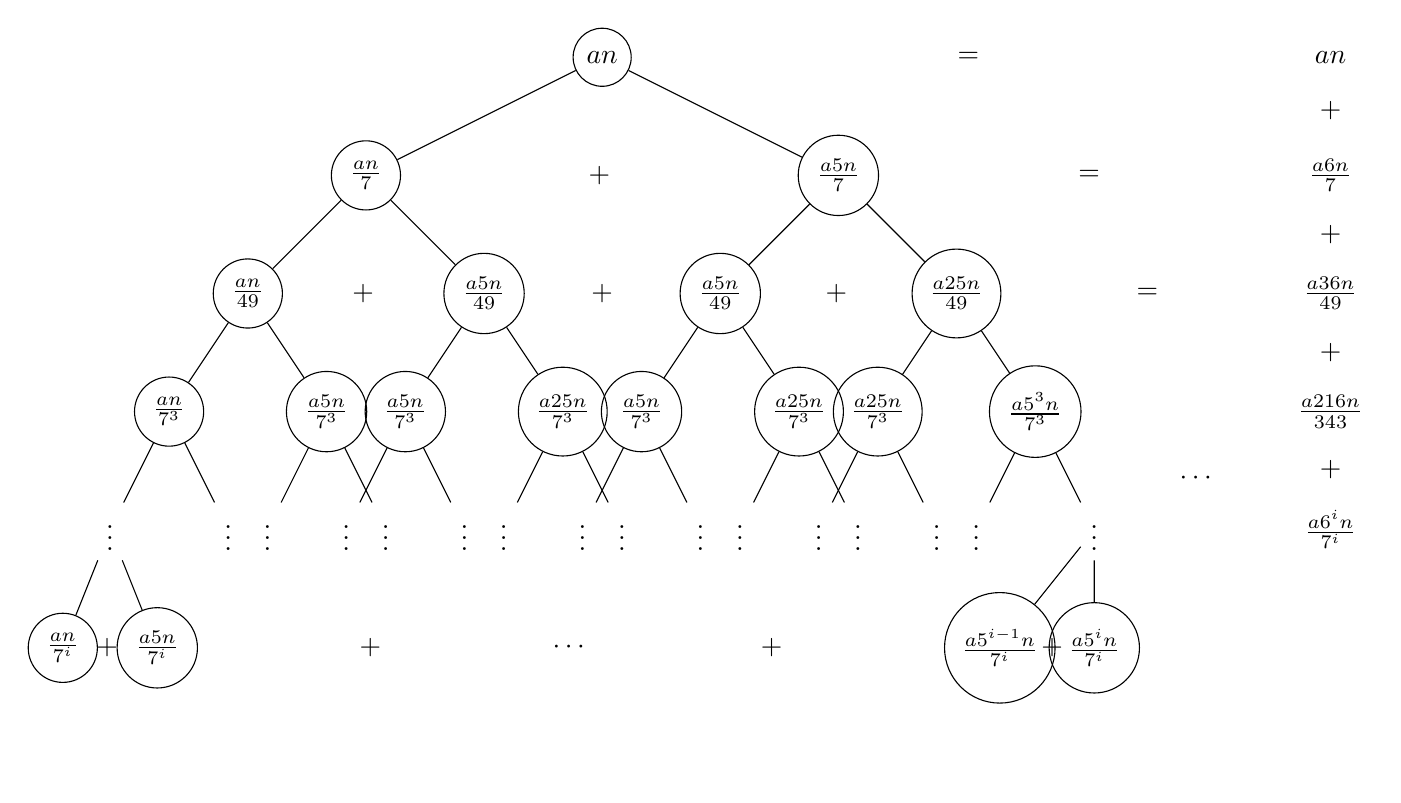
\begin{tikzpicture}[level/.style={sibling distance=60mm/#1}]
\node [circle,draw] (z){$an$}
  child {node [circle,draw] (a) {$\frac{an}{7}$}
    child {node [circle,draw] (b) {$\frac{an}{49}$}
      child {node [circle,draw] (bl) {$\frac{an}{7^3}$}
        child {node {$\vdots$}
          child {node [circle,draw] (d) {$\frac{an}{7^i}$}}
          child {node [circle,draw] (e) {$\frac{a5n}{7^i}$}}
          }
        child {node {$\vdots$}}
        }
      child {node [circle,draw] (br) {$\frac{a5n}{7^3}$}
        child {node {$\vdots$}}
        child {node {$\vdots$}}
        }
      } 
    child {node [circle,draw] (g) {$\frac{a5n}{49}$}
      child {node [circle,draw] (gl) {$\frac{a5n}{7^3}$}  
        child {node {$\vdots$}}
        child {node {$\vdots$}}
      }
      child {node [circle,draw] (gr) {$\frac{a25n}{7^3}$}  
        child {node {$\vdots$}}
        child {node {$\vdots$}}
      }
    }
  }
  child {node [circle,draw] (j) {$\frac{a5n}{7}$}
    child {node [circle,draw] (k) {$\frac{a5n}{49}$}
      child {node [circle,draw] (kl) {$\frac{a5n}{7^3}$}
        child {node {$\vdots$}}
        child {node {$\vdots$}}
      }
      child {node [circle,draw] (kr) {$\frac{a25n}{7^3}$}
        child {node {$\vdots$}}
        child {node {$\vdots$}}  
      }
    }
    child {node [circle,draw] (l) {$\frac{a25n}{49}$}
      child {node [circle,draw] (ll) {$\frac{a25n}{7^3}$}
        child {node {$\vdots$}}
        child {node {$\vdots$}}
      }	
      child {node [circle,draw] (lr) {$\frac{a5^3n}{7^3}$}
        child {node {$\vdots$}}
        child {node (c){$\vdots$}
          child {node [circle,draw] (o) {$\frac{a5^{i-1}n}{7^i}$}}
          child {node [circle,draw] (p) {$\frac{a5^in}{7^i}$}}
            child [grow=right] {node (q) {$  $} edge from parent[draw=none]
              child [grow=right] {node (q) {$\frac {a6^in}{7^i}$} edge from parent[draw=none]
                child [grow=up] {node (r) {$\frac{a216n}{343}$} edge from parent[draw=none]
                  child [grow=up] {node (s) {$ \frac{a36n}{49}$} edge from parent[draw=none]
                    child [grow=up] {node (t) {$\frac{a6n}7$} edge from parent[draw=none]
                      child [grow=up] {node (u) {$ an $} edge from parent[draw=none]}
                }
              }
            }
            child [grow=down] {node (v) {$$}edge from parent[draw=none]}
          }
        }
      }
    }
  }
};
\path (a) -- (j) node [midway] {+};
\path (b) -- (g) node [midway] {+};
\path (k) -- (l) node [midway] {+};
\path (k) -- (g) node [midway] {+};
\path (d) -- (e) node [midway] {+};
\path (o) -- (p) node [midway] {+};
\path (o) -- (e) node (x) [midway] {$\cdots$}
  child [grow=down] {
    node (y) {$$}
    edge from parent[draw=none]
  };
\path (q) -- (r) node [midway] {+};
\path (s) -- (r) node [midway] {+};
\path (s) -- (t) node [midway] {+};
\path (s) -- (l) node [midway] {=};
\path (t) -- (u) node [midway] {+};
\path (z) -- (u) node [midway] {=};
\path (j) -- (t) node [midway] {=};
\path (y) -- (x) node [midway] {$$};
\path (v) -- (y)
  node (w) [midway] {$$};
\path (q) -- (v) node [midway] {};
\path (e) -- (x) node [midway] {+};
\path (o) -- (x) node [midway] {+};
\path (y) -- (w) node [midway] {};
\path (v) -- (w) node [midway] {$$};
\path (r) -- (c) node [midway] {$\cdots$};
\end{tikzpicture}\\

The point of this messy picture is to show that at increasing levels of the recursion tree, we have decreasing costs. Waving our hands a bit, we can see that this is happening as the denominator of each level's costs is multiplied by 7, while the numerator, as levels increase, is outpaced by the denominator. Intuitively, and from our knowledge of the Master Theorem, if the costs are dominated at the root, then we will have case 3. Obviously the MT can't be applied to this situation formally, but we can observe that $an$ is the largest cost, and we have decreasing costs all the way down until we've run out of inputs to the problem. We know from our proof of the 5-groups version of this problem that the fractions of the recurrences to this problem break down to an infinite geometric series that, in closed form, evaluates to a constant multiplied by the costs incurred by dividing and conquering, which we know are $O(n)$. In other words, dividing the problem into groups of 7 also $\in O(n)$.\\\\
Looking at this a bit more formally, we can see that the right node of the rightmost branch of each level of the recursion tree is always the node that contains the largest subproblem (this is the only branch where the 5 in the numerator is raised to the same power as the 7 in the denominator) and therefore incurs the largest cost for each level. Therefore, if there are $i$ levels on this unlucky side, then this subtree will be greater than or equal to all subtrees to the left of it (in height), because the problem size will approach zero more quickly for smaller subproblems (subtrees from leftmost to right). We can set $T(1) = 1$ as our base case for this rightmost subtree, and solving: 

\begin{align*}
T(1) &= T(n\frac {5^i}{7^i})\\
1 &= n\frac {5^i}{7^i}\\
\frac 1n &= \frac {5^i}{7^i}\\
n &= \frac{7^i}{5^i}\\
n &= (\frac 75)^i\\
i &= \log_{\frac 75}n
\end{align*}\\

This tells us that we will need to recursively call this algorithm at most log$_\frac75n$ times. So, we could consider the just costs at the rightmost node for each level from the root to the rightmost leaf of a tree of height log$_\frac75n$:

\begin{align*}
&an\sum_{i=0}^{\log_{\frac75}n}\frac{5^i}{7^i}\\
&= an\sum_{i=0}^{\log_{\frac75}n}(\frac{5}{7})^i\\
&= an \cdot \frac{1-\frac57^{\log_{\frac75}n+1}}{1-\frac57}\\
&= an \cdot \frac72 \cdot(1 -\frac57^{\log_{\frac75}n+1})\\
&= an \cdot \frac72 \cdot(1 -\frac57^{\log_{\frac75}n}\cdot(\frac 57))\\
&= an \cdot \frac72 \cdot(1 - \frac75^{-1^{\log_{\frac75}n}}\cdot\frac 57)\\
&= an \cdot \frac72 \cdot(1- \frac75^{\log_{\frac75}n^-1}\cdot\frac 57)\\
&= an \cdot \frac72 \cdot(1- \frac75^{\log_{\frac75}\frac 1n}\cdot\frac 57)\\
&= an \cdot \frac72 \cdot(1- \frac1n\cdot\frac 57)\\
&= an \cdot \frac72 \cdot(1- \frac5{7n})\\
&= an \cdot \Big(\frac72-\frac72\cdot \frac 5{7n}\Big)\\
&= an \cdot \Big(\frac72-\frac5{2n}\Big)\\
&= \frac {an7}2-\frac {an5}{2n}\\
&= \frac {an7}2 -\frac {a5}2\\
&= \frac {a(n7-5)}2\\
&= 3.5an\\
&= O(n)
\end{align*}\\

We know from the recursion tree that this branch incurs the highest cost of this tree, and even after adding the other costs (small fractions of $n$) we will still have a result in linear time.   

To illustrate more clearly the weight of the right we could recognize that the costs at each level add up to $an\frac {6^i}{7^i}$ and set $i = \log_{\frac76}n$. We can derive a similar solution by summing all the levels to get a constant multiplied by $an$ to discover the total costs:

\begin{align*}
&an\sum_{i=0}^{\log_{\frac76}n}\frac{6^i}{7^i}\\
&= an\sum_{i=0}^{\log_{\frac76}n}(\frac{6}{7})^i\\
&= an \cdot \frac{1-\frac67^{\log_{\frac76}n+1}}{1-\frac67}\\
&= an \cdot 7 \cdot(1 -\frac67^{\log_{\frac76}n+1})\\
&= an \cdot 7 \cdot(1 -\frac67^{\log_{\frac76}n}\cdot(\frac 67))\\
&= an \cdot 7 \cdot(1 - \frac76^{-1^{\log_{\frac76}n}}\cdot\frac 67)\\
&= an \cdot 7 \cdot(1- \frac76^{\log_{\frac76}n^-1}\cdot\frac 67)\\
&= an \cdot 7 \cdot(1- \frac76^{\log_{\frac76}\frac 1n}\cdot\frac 67)\\
&= an \cdot 7 \cdot(1- \frac1n\cdot\frac 67)\\
&= an \cdot 7 \cdot(1- \frac6{7n})\\
&= an \cdot \Big(7-7\cdot \frac 6{7n}\Big)\\
&= an \cdot \Big(7-\frac6{n}\Big)\\
&= an7-\frac {an6}{n}\\
&= an7 - a6\\
&= a(n7-6)\\
&= 7an\\
&= O(n)
\end{align*}\\  

It looks like the rightmost branch of the tree costs roughly half of the total cost at each level for sufficiently large $n$, which is an interesting result. 

\subparagraph{(b) [10 points]}
Show that groups of size 3 results in superlinear time complexity.\\\\
This instance of the problem is actually super interesting, because you would imagine that, like the groups of 5 or 7, it would also have linear time complexity. Let's jump right in and then discuss after, using the same logic as above to determine elements larger than x pre-`mom': \\

\begin{align*}
2 \Bigg( \ceil[Bigg]{\frac 12} \cdot \ceil[Big]{\frac n3} -2 \Bigg) \geq \frac {n}{3} -4
\end{align*}\\

Again, the complexity is similar for the first stage of the algorithm. Copying and pasting, it takes constant time to call insertion sort on all of the groups of 3 elements, but we'd have to call it $O(n)$ times, plus the constant factor of splitting into groups of 3; all of this would cost $\ceil[big]{\frac n3} +an$. The recurrence: 

\begin{align*}
T(n) &= T(\frac n3) + T(\frac {2n}3)+4+an\\ 
\end{align*} 

Ditch the 4 and let's climb down the tree once again:



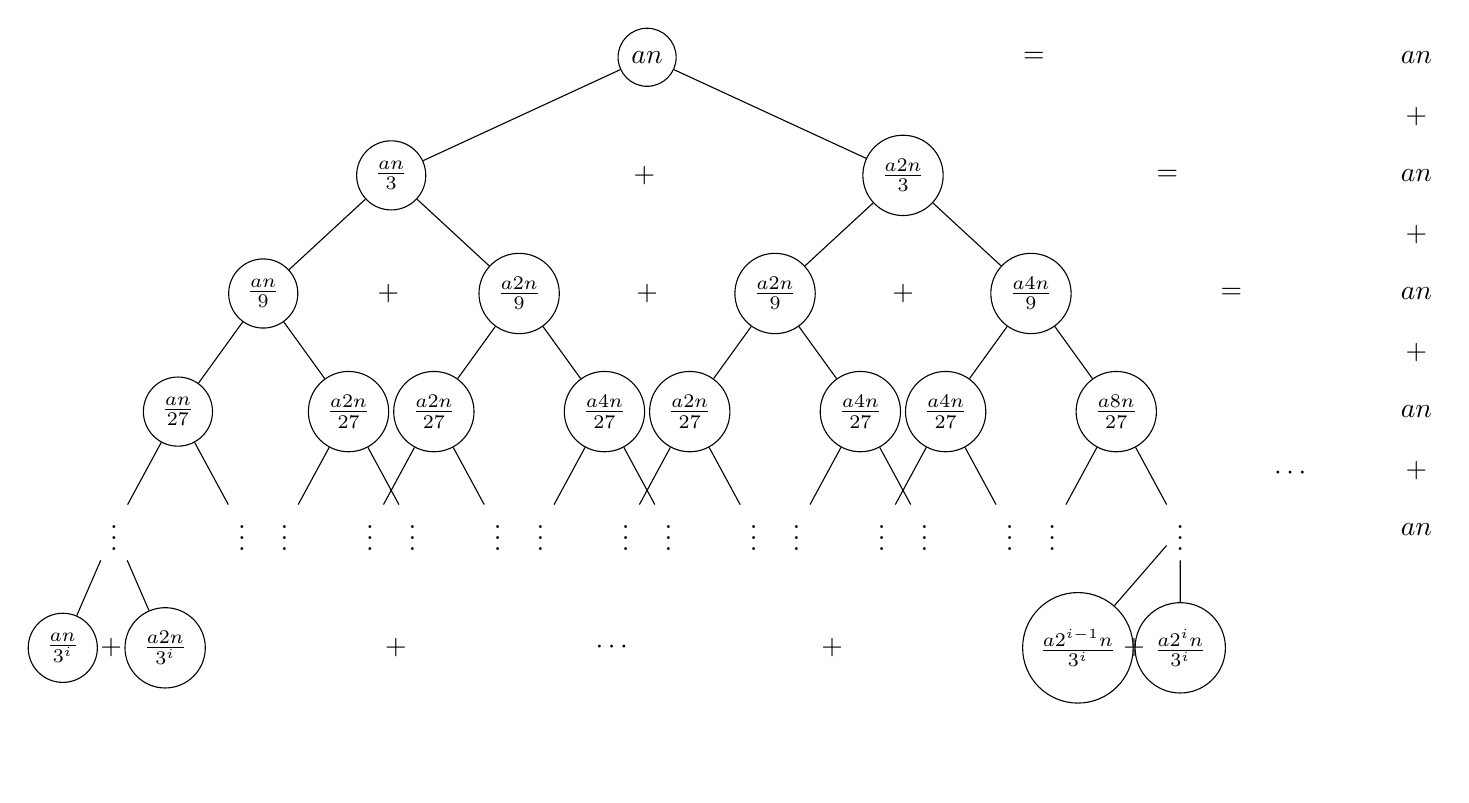
\begin{tikzpicture}[level/.style={sibling distance=65mm/#1}]
\node [circle,draw] (z){$an$}
  child {node [circle,draw] (a) {$\frac{an}{3}$}
    child {node [circle,draw] (b) {$\frac{an}{9}$}
      child {node [circle,draw] (bl) {$\frac{an}{27}$}
        child {node {$\vdots$}
          child {node [circle,draw] (d) {$\frac{an}{3^i}$}}
          child {node [circle,draw] (e) {$\frac{a2n}{3^i}$}}
          }
        child {node {$\vdots$}}
        }
      child {node [circle,draw] (br) {$\frac{a2n}{27}$}
        child {node {$\vdots$}}
        child {node {$\vdots$}}
        }
      } 
    child {node [circle,draw] (g) {$\frac{a2n}{9}$}
      child {node [circle,draw] (gl) {$\frac{a2n}{27}$}  
        child {node {$\vdots$}}
        child {node {$\vdots$}}
      }
      child {node [circle,draw] (gr) {$\frac{a4n}{27}$}  
        child {node {$\vdots$}}
        child {node {$\vdots$}}
      }
    }
  }
  child {node [circle,draw] (j) {$\frac{a2n}{3}$}
    child {node [circle,draw] (k) {$\frac{a2n}{9}$}
      child {node [circle,draw] (kl) {$\frac{a2n}{27}$}
        child {node {$\vdots$}}
        child {node {$\vdots$}}
      }
      child {node [circle,draw] (kr) {$\frac{a4n}{27}$}
        child {node {$\vdots$}}
        child {node {$\vdots$}}  
      }
    }
    child {node [circle,draw] (l) {$\frac{a4n}{9}$}
      child {node [circle,draw] (ll) {$\frac{a4n}{27}$}
        child {node {$\vdots$}}
        child {node {$\vdots$}}
      }	
      child {node [circle,draw] (lr) {$\frac{a8n}{27}$}
        child {node {$\vdots$}}
        child {node (c){$\vdots$}
          child {node [circle,draw] (o) {$\frac{a2^{i-1}n}{3^i}$}}
          child {node [circle,draw] (p) {$\frac{a2^in}{3^i}$}}
            child [grow=right] {node (q) {$  $} edge from parent[draw=none]
              child [grow=right] {node (q) {$an$} edge from parent[draw=none]
                child [grow=up] {node (r) {$an$} edge from parent[draw=none]
                  child [grow=up] {node (s) {$an$} edge from parent[draw=none]
                    child [grow=up] {node (t) {$an$} edge from parent[draw=none]
                      child [grow=up] {node (u) {$ an $} edge from parent[draw=none]}
                }
              }
            }
            child [grow=down] {node (v) {$$}edge from parent[draw=none]}
          }
        }
      }
    }
  }
};
\path (a) -- (j) node [midway] {+};
\path (b) -- (g) node [midway] {+};
\path (k) -- (l) node [midway] {+};
\path (k) -- (g) node [midway] {+};
\path (d) -- (e) node [midway] {+};
\path (o) -- (p) node [midway] {+};
\path (o) -- (e) node (x) [midway] {$\cdots$}
  child [grow=down] {
    node (y) {$$}
    edge from parent[draw=none]
  };
\path (q) -- (r) node [midway] {+};
\path (s) -- (r) node [midway] {+};
\path (s) -- (t) node [midway] {+};
\path (s) -- (l) node [midway] {=};
\path (t) -- (u) node [midway] {+};
\path (z) -- (u) node [midway] {=};
\path (j) -- (t) node [midway] {=};
\path (y) -- (x) node [midway] {$$};
\path (v) -- (y)
  node (w) [midway] {$$};
\path (q) -- (v) node [midway] {};
\path (e) -- (x) node [midway] {+};
\path (o) -- (x) node [midway] {+};
\path (y) -- (w) node [midway] {};
\path (v) -- (w) node [midway] {$$};
\path (r) -- (c) node [midway] {$\cdots$};
\end{tikzpicture}\\

Unfortunately, we have a curious problem here. Namely, each level of recursion incurs the exact same cost of $an$. This is similar to situations that correspond to Master Theorem case 2. Again, we can't use the MT, but we can observe that at all levels of the tree the costs are evenly split and therefore we can't, like above, take the root's costs and ignore the rest of the tree. Instead, we must take the costs of all of the levels of recursion. How far does this tree go down? Using the same logic as above, the rightmost subtree's leaves are at $T(1)=1$ and $i = $log$_{\frac32}n$. We don't really need to perform the summation\\

\begin{align*}
\sum_{i=0}^{\log_{\frac32}n}an
\end{align*} this time because we can see that this will cost us around $an \log_{\frac32}n$ so this is (as we would expect for MT case 2 as well) $\in O(n \>log \>n)$.

\end{document}